\documentclass[conference]{IEEEtran}
\IEEEoverridecommandlockouts
% The preceding line is only needed to identify funding in the first footnote. If that is unneeded, please comment it out.
\usepackage{cite}
\usepackage{amsmath,amssymb,amsfonts}
\usepackage{algorithmic}
\usepackage{graphicx}
\usepackage{textcomp}
\usepackage{xcolor}
\usepackage[brazilian]{babel}
\usepackage[utf8]{inputenc}
\usepackage[T1]{fontenc}
\usepackage{listings}
\usepackage{color}
\usepackage{float}
\usepackage{multirow}

\definecolor{dkgreen}{rgb}{0,0.6,0}
\definecolor{gray}{rgb}{0.5,0.5,0.5}
\definecolor{mauve}{rgb}{0.58,0,0.82}

\lstset{frame=tb,
  language=Java,
  aboveskip=3mm,
  belowskip=3mm,
  showstringspaces=false,
  columns=flexible,
  basicstyle={\small\ttfamily},
  numbers=none,
  numberstyle=\tiny\color{gray},
  keywordstyle=\color{blue},
  commentstyle=\color{dkgreen},
  stringstyle=\color{mauve},
  breaklines=true,
  breakatwhitespace=true,
  tabsize=3
}
\lstset{language=Python}
\def\BibTeX{{\rm B\kern-.05em{\sc i\kern-.025em b}\kern-.08em
    T\kern-.1667em\lower.7ex\hbox{E}\kern-.125emX}}
\begin{document}

\title{Relatório do Laboratório 3: \\ Otimização com Métodos de Busca Local\\
}

\author{\IEEEauthorblockN{Isabelle Ferreira de Oliveira}
\IEEEauthorblockA{\textit{CT-213 - Engenharia da Computação 2020} \\
\textit{Instituto Tecnológico de Aeronáutica (ITA)}\\
São José dos Campos, Brasil \\
isabelle.ferreira3000@gmail.com}
}

\maketitle

\begin{abstract}
Esse relatório documenta a implementação dos seguintes algoritmos de otimização baseados em busca local: Descida do Gradiente, Hill Climbing e Simulated Annealing. Esses métodos foram testados em uma regressão linear para obter parâmetros físicos relativos ao movimento de uma bola. Por fim, os resultados das três implementações foram comparados.
\end{abstract}

\begin{IEEEkeywords}
Algoritmos de Otimização, busca local, Descida de Gradiente, Hill Climbing, Simulated Annealing, regressão linear
\end{IEEEkeywords}

\section{Introdução}
Planejamento de ações de agentes podem ser implementados por diversos métodos atualmente. Construindo-se um grafo que represente diferentes opções de estados para o agente, por exemplo, um planejamento de ação pode ser definido aplicando um algoritmo de busca em grafo, partindo da situação inicial do agente até o estado desejado, onde cada aresta representa uma possível ação, atrelada a um custo para executá-la.

Seguindo esse contexto, para decidir qual melhor planejamento a se escolher (considerando que essa escolha é baseada em menor custo de se sair de uma situação de início para um objetivo), pode-se aplicar algoritmos de busca de caminho mínimo, como Dijkstra, Greedy (ou Guloso) e A*. 

Os pseudo-códigos desses algoritmos podem ser vistos nas subseções a seguir. Em seguida, será apresentado como esses algoritmos foram implementados no contexto do laboratório.

\subsection{Algoritmo de Dijkstra}
\begin{lstlisting}
dijkstra(start):
	pq = PriorityQueue()
	start.cost = 0
	pq.insert_or_update(start.cost, start)
	while not pq.empty():
		node = pq.extract_min()
		for successor in node.successors():
			if successor.cost > node.cost + cost(node, successor):
				successor.cost = node.cost + cost(node, successor)
				successor.parent = node
				pq.insert_or_update(successor.cost, node)
\end{lstlisting}

\subsection{Algoritmo Greedy}
\begin{lstlisting}
greedy_search(start, goal):
	pq = PriorityQueue()
	start.cost = h(start, goal)
	pq.insert_or_update(start.cost, start)
	while not pq.empty():
		node = pq.extract_min()
		for successor in node.successors():
			successor.parent = node
			if successor.content == goal:
				return successor
			successor.cost = h(successor, goal)
			pq.insert_or_update(successor.cost, successor)
\end{lstlisting}

\subsection{Algoritmo A*}
\begin{lstlisting}
a_star(start, goal):
	pq = PriorityQueue()
	start.g = 0
	start.f = h(start, goal)
	pq.insert_or_update(start.f, start)
	while not pq.empty():
		node = pq.extract_min()
		if node.content == goal:
			return successor
		for successor in node.successors():
			if successor.f > node.g + cost(node, successor) + h(successor, goal):
				successor.g = node.g + cost(node, successor)
				successor.f = successor.g + h(successor, goal)
				successor.parent = node
				pq.insert_or_update(successor.f, successor)
\end{lstlisting}

\section{Implementação dos algoritmos}
Na parte relativa a implementação dos algoritmos de busca, era necessário preencher os códigos das funções \textit{dijkstra}, \textit{greedy} e \textit{a\underline{\space}star} da classe \textit{PathPlanner} do código base fornecido \cite{b1}.

A análise de vários pontos dos algoritmos descritos acima terão uma breve descrição em alto nível da sua implementação a seguir. 

Como os algoritmos foram implementados em Python, as filas de prioridade foram importadas da biblioteca \textit{heapq}, sendo utilizado as funções \textit{heappush} e \textit{heappop} para adicionar e retirar um elemento da fila, respectivamente.

Já as funções heurísticas dos algoritmos Greedy e A* foram calculadas a partir da função \textit{distance\underline{\space}to}, que calcula a distância euclidiana entre um nó específico e o nó objetivo. Essa função já foi fornecida pelo código básico.

Na etapa de percorrer os sucessores de um determinado nó para se calcular os custos relativos aquele caminho analisado, utilizou-se a função \textit{get\underline{\space}successors} para se obter esses sucessores. Para cada nó analisado, então, seu nó sucessor foi adicionado à fila de prioridade, sendo o custo dependente se o movimento se deu pela diagonal ou pela lateral do nó do \textit{grid}. Dessa forma, passos laterais tiveram custos menores que passos diagonais, na proporção de 1:$\sqrt{2}$. Uma representação de um nó específico do grafo e seus 8 vizinhos foi apresentado na Figura \ref{8-conectado}.

\begin{figure}[htbp]
\centerline{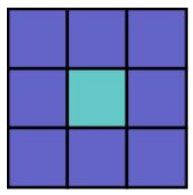
\includegraphics[scale=0.4]{8-conectado.png}}
\caption{Representação de 8-conectado. Cada nó apresenta 8 vizinhos, sendo 4 laterais e 8 diagonais.}
\label{8-conectado}
\end{figure}

Quando um determinado nó era, por fim, retirado da fila de prioridade, o custo mínimo do início do trajeto até aquele ponto já estaria definido. Nesse instante, então, o atributo \textit{closed} daquele nó foi setado como \textit{True}. Ao nó com custo definido de caminho do início até ele for o nó objetivo, a busca encerrou-se. No algoritmo Greedy, excepcionalmente, o custo já estava definido desde a primeira vez que o nó em específico era visitado.

\section{Resultados e Conclusões}
Os resultados obtidos após 1 execução das implementações dos algoritmos descritos acima foram apresentados nas Figuras \ref{dijkstra}, \ref{greedy} e \ref{a_star} para Dijkstra, Greedy e A*, respectivamente.

Foi executado também 100 vezes cada um dos códigos, para se calcular as médias e as variâncias dos custos de tempo computacional e de caminho para os três algoritmos, e os resultados foram apresentados na Tabela \ref{tabelaX}.

\begin{figure}[htbp]
\centerline{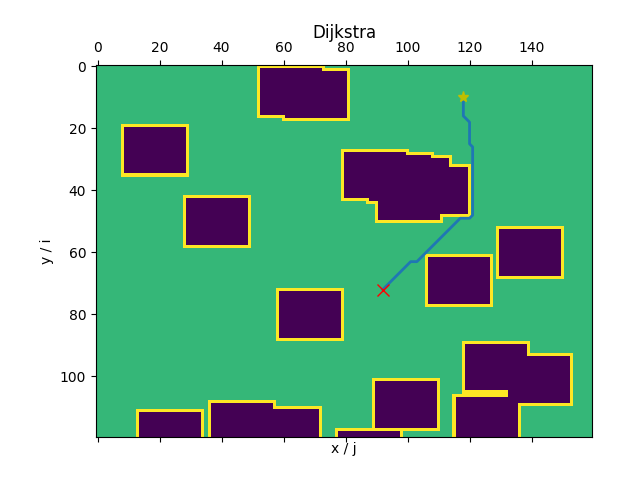
\includegraphics[scale=0.4]{dijkstra_0.png}}
\caption{Execução do algoritmo de Dijkstra para busca do caminho mínimo no grafo em grid do laboratório.}
\label{dijkstra}
\end{figure}

\begin{figure}[htbp]
\centerline{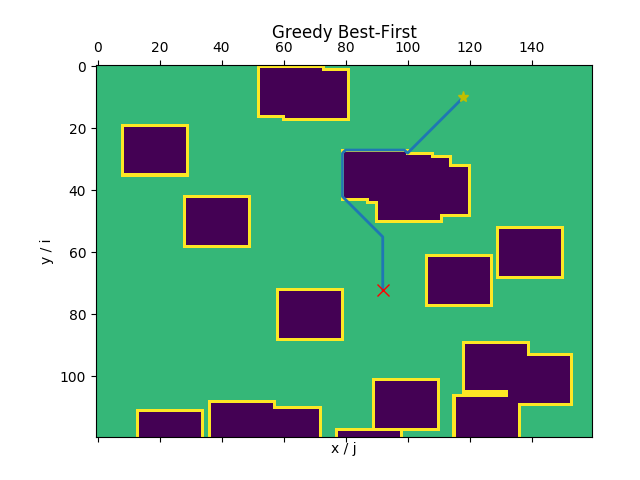
\includegraphics[scale=0.4]{greedy_0.png}}
\caption{Execução do algoritmo Greedy para busca do caminho mínimo no grafo em grid do laboratório.}
\label{greedy}
\end{figure} 

\begin{figure}[htbp]
\centerline{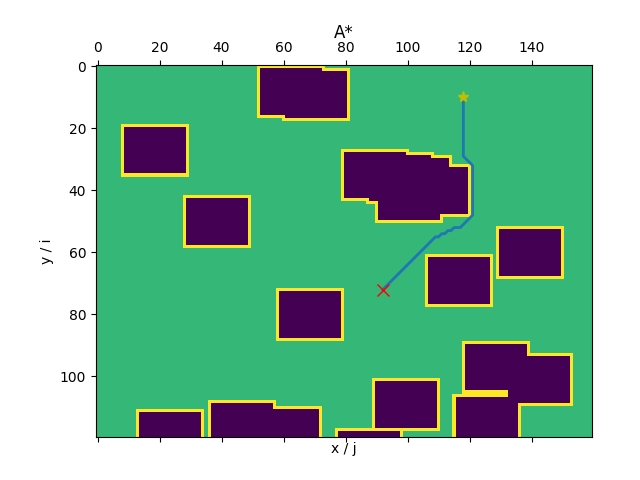
\includegraphics[scale=0.4]{a_star_0.png}}
\caption{Execução do algoritmo A* para busca do caminho mínimo no grafo em grid do laboratório.}
\label{a_star}
\end{figure}

\begin{table}[H]
\caption{Comparação dos custos de tempo computacional e custos de caminho para os algoritmos do laboratório.}
\label{tabelaX}
\begin{tabular}{cc|c|c|c|c|l}
\cline{1-5}
\multicolumn{1}{ |c  }{\multirow{2}{*}{\textbf{Algoritmo}}} & 
\multicolumn{2}{ |c  }{\textbf{Tempo Computacional (s)}} &
\multicolumn{2}{ |c| }{\textbf{Custo do caminho}}
\\ \cline{2-5}
\multicolumn{1}{ |c  }{} & 
\multicolumn{1}{ |c  }{\textbf{Média}} & 
\multicolumn{1}{ |c  }{\textbf{Desvio Padrão}} & 
\multicolumn{1}{ |c  }{\textbf{Média}} & 
\multicolumn{1}{ |c| }{\textbf{Desvio Padrão}}
\\ \cline{1-5} 
\multicolumn{1}{ |c  }{Dijkstra} &
\multicolumn{1}{ |c  }{0.2796} &
\multicolumn{1}{ |c  }{0.1616} &
\multicolumn{1}{ |c  }{79.8291} &
\multicolumn{1}{ |c| }{38.5709}
\\ \cline{1-5}
\multicolumn{1}{ |c  }{Greedy Search} &
\multicolumn{1}{ |c  }{0.03101} &
\multicolumn{1}{ |c  }{0.0864} &
\multicolumn{1}{ |c  }{175.9340} &
\multicolumn{1}{ |c| }{91.9683}
\\ \cline{1-5}
\multicolumn{1}{ |c  }{A*} &
\multicolumn{1}{ |c  }{0.3112} &
\multicolumn{1}{ |c  }{0.2100} &
\multicolumn{1}{ |c  }{79.8291} &
\multicolumn{1}{ |c| }{38.5709}
\\ \cline{1-5}

\end{tabular}
\end{table}

Isso era esperado, uma vez que, os custos de caminho dos algoritmos de Dijkstra e A* são equivalentes (ambos ótimos), e o do Greedy é significantemente maior. Além disso, os tempos computacionais são crescentes na ordem dos algoritmos Greedy, A* e Dijkstra.

\begin{thebibliography}{00}
\bibitem{b1} M. Maximo, ``Roteiro: Laboratório 2 - Busca Informada''. Instituto Tecnológico de Aeronáutica, Departamento de Computação. CT-213, 2019.
\end{thebibliography}

\end{document}
